\section{Implementation}\label{sec:implementation}

To implement \sysname{}, we use the basic match-action functionality that is
available in most modern commodity switches. However, correct implementation
requires a key insight into the way PFC PAUSE frames are handled.

\begin{figure}
	\hspace{-0.2in}
	\centering
	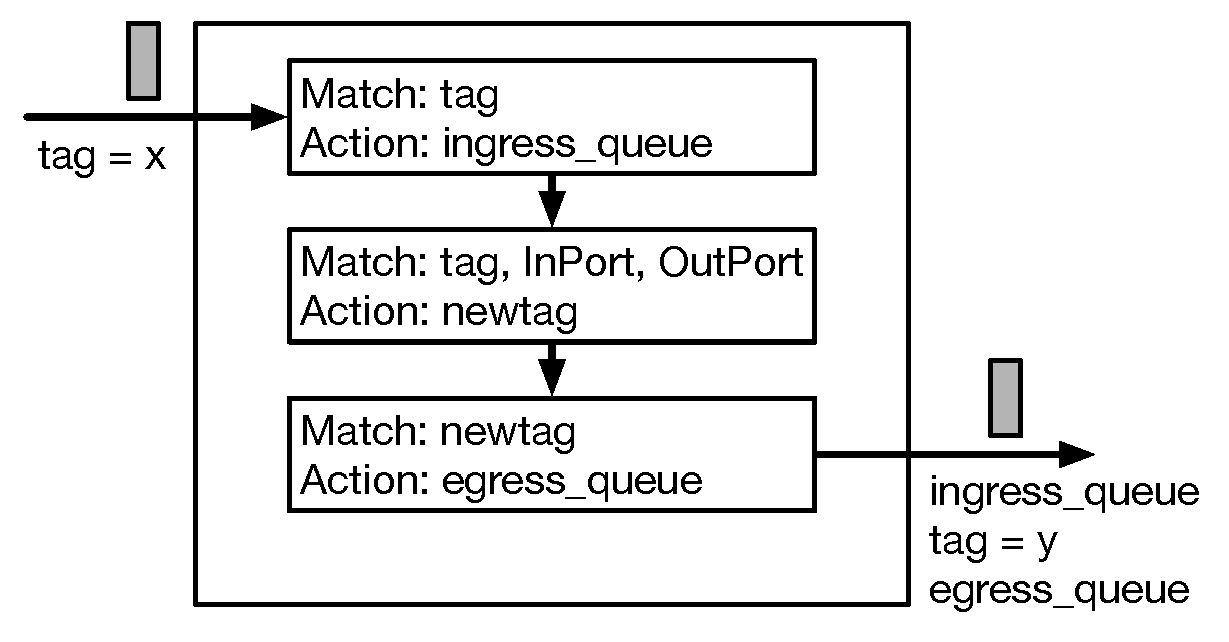
\includegraphics[width=0.5\textwidth] {figs/Tagger}
	\caption{Tagger match-action rules}\label{fig:tagger}
	
\end{figure}

\para {Match-Action rules:} \sysname{} needs to perform two operations at every
hop in the network, i.e., {\em tag-based priority queueing} and {\em tag
rewriting}.  These two operations are implemented using a 3-step match-action
pipelines shown in Figure~\ref{fig:tagger}.  In the first step, \sysname{}
classifies packets into ingress queues based on the value of tags. In the second
step, \sysname{} rewrites the value of tag based on (tag, inport, outport)
information. These two steps form the core of \sysname{}.

\begin{figure}[t]
 	\centering
 	\subfloat[short for lof][Ingress priority = egress priority  $\rightarrow$ packet drop.] {
 		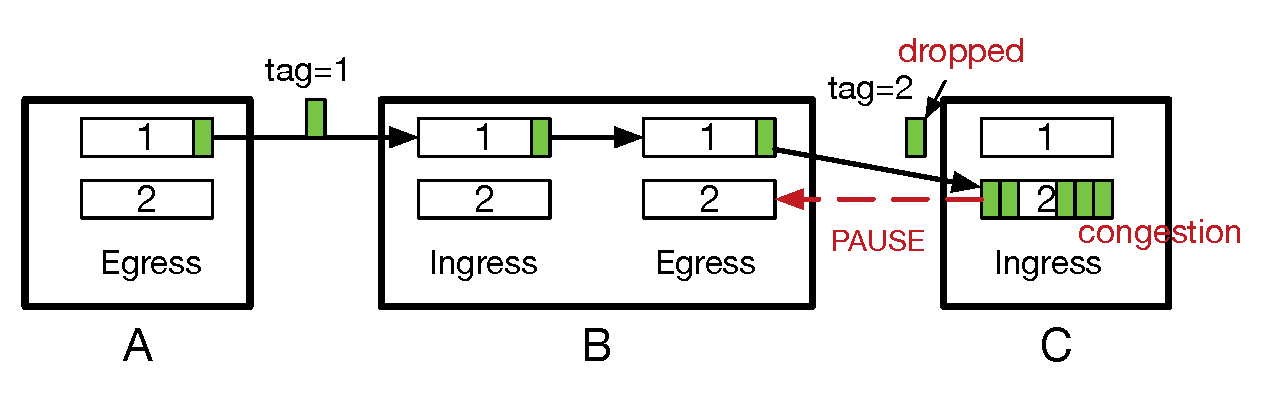
\includegraphics[width=0.43\textwidth] {figs/prioritydecoupling_1}
 	}

 	\subfloat[short for lof][Ingress priority = 1, egress priority = 2 $\rightarrow$ no drop.]{
 		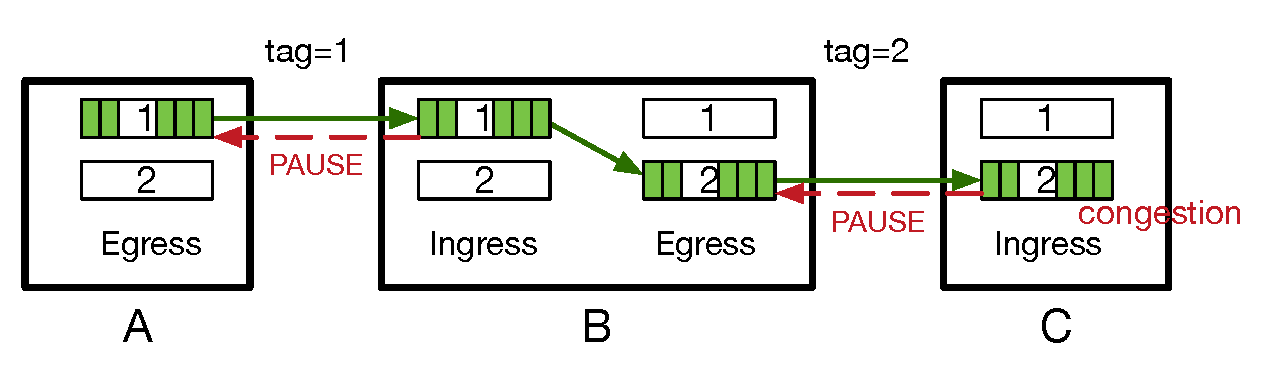
\includegraphics[width=0.43\textwidth] {figs/prioritydecoupling_2}
 	}
 	\caption{Decoupling ingress priority from egress priority at switch B is necessary for lossless priority transition.}\label{fig:prioritydecoupling}
	\vspace{-1em}
\end{figure}

\para{Handling priority transition:}
{\em The third step, wherein the packet is placed in an egress queue based on the
{\em new} tag value, is needed to ensure correct PFC operation when priority
values are rewritten.}

Note that the tagged graph $G$ only defines the mapping between tags and ingress
queues. By default, a switch will enqueue a departing packet in the egress queue
of the same priority class as its ingress queue. This default behavior can lead
to packet loss when priority transition is performed. An example is shown in
Figure~\ref{fig:prioritydecoupling}.

In this example, switch B is configured to do priority transition for packets
received from switch A and destined for switch C. It is important to note that
in this diagram, only {\em one port} on each switch is active. The two queues
are for two priorities.

In Figure~\ref{fig:prioritydecoupling}(a), we consider the default behavior.
Packets exit egress queue 1 at switch B, but with priority 2.  This can lead to
to packet loss when ingress queue 2 of switch C becomes congested, because
the PFC PAUSE from switch C to switch B carries priority 2, and cannot pause
the offending egress queue 1 of switch B.

In Figure~\ref{fig:prioritydecoupling}(b), we map the packet to the egress queue
based on its new priority.  This avoids packet loss, since the PFC from switch C
correctly pauses the queue on which the packet with the new tag would be
exiting. This example thus demonstrates the necessity of the third step.

\para{Rule compression:}  The match-action rules of \sysname{}
are implemented with TCAM. TCAM entries consist of three parts ({\em Pattern},
{\em Mask}, {\em Result}). {\em Pattern} refers to the pattern to be matched, {\em
Mask} refers to the mask bits associated with the pattern and {\em Result}
refers to the action that occurs when a lookup hits the pattern.  One TCAM entry
can have several Pattern-Mask pairs to match multiple packet header fields
simultaneously, e.g., an entry like (Pattern-1, Mask-1, Pattern-2, Mask-2, Result)
matches two fields simultaneously and fires only if both matches succeed.

\begin{figure}
	\centering
	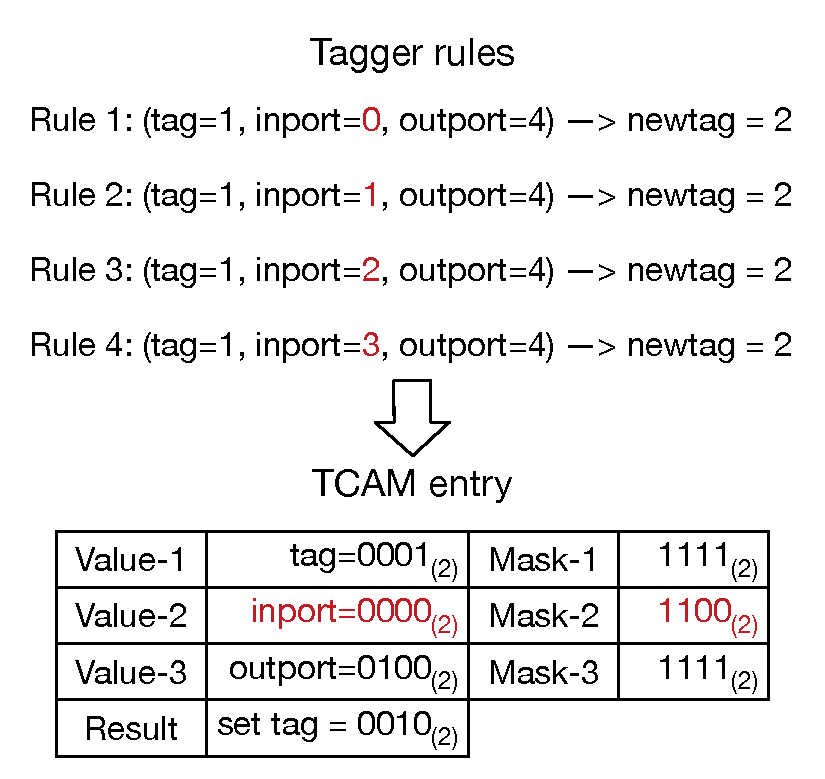
\includegraphics[width=0.45\textwidth] {figs/compression_with_bitmasking}
	\caption{Rule compression with bit masking.}\label{fig:compression}
    \vspace{-1em}	
\end{figure}

Rules that have the same action can be compressed into one TCAM entry, if the
patterns to be matched can be aggregated using bit masking. Consider the three
rules in Figure~\ref{fig:compression}. These rules share the same tag value,
egress port and tag rewriting action.

Note that port numbers in TCAM are bitmaps, and not binary values. To match a single port, we can simply set the corresponding bit in the pattern to 1, and set the mask to all 1s. 

However, in order to match multiple ports with one rule, we should set the pattern to all 0s, and set the corresponding bits in the mask to 0. As shown in Figure~\ref{fig:compression},  to match ingress ports 0, 1 and 3, we set Pattern-2 to ``0000''  and Mask-2 to ``0100''. In this case, only the packet received from ingress port 0, 1 or 3 will match Pattern-2 after doing bit masking with Mask-2. Thus, the three \sysname{} rules are compressed into
a single TCAM entry.

Recall from \S\ref{sec:generic} that without any compression, we need
$n(n-1)m(m-1)/2$ rules per switch. The number of rules can be
compressed to $nm(m-1)/2$ by aggregating ingress ports.  The
result can be further improved by doing joint aggregation on tag, ingress port and
egress port.

\para{Broadcom implementation:} We have implemented \sysname{} on commodity
switches based on Broadcom chipsets.  We use DSCP field in IP header as the tag.
DSCP rewriting is supported by all commodity chipsets. DSCP-based priority
queuing (step 1) is supported natively by all switch ASIC vendors. Step 2 uses
ingress ACL rules to map (DSCP, inport, outport) to new DSCP.

Step 3 also uses ACLs, although it relies on certain details that are specific
to Broadcom's match-action pipeline. We omit these gritty details for brevity.
While the implementation of this step is Broadcom-specific, we believe that
ASICs from other vendors can also support this functionality.

%%comment: this claim is not true, as brcm sdk is never public.
%%         
We stress that none of the three steps require any changes to the switch ASIC,
and everything is implemented using publicly available and documented
functionality.

We considered using TTL instead of DSCP to tag packets, but TTL is decremented
by the forwarding pipeline, which complicates the rule structure.

